\section{The actuator disks}
As mentioned, there is no standard way of designing \gls{AD}s. For this project, it was desirable to create \gls{AD}s with multiple solidities, and a possible method was to create two \gls{AD}s that are connected and can be rotated relative to each other, in order to change the solidity. However, this seemed hard to achieve at such small scales. In addition, the author was skeptic to the method based on the results of Pierella et al (2010) \cite{Pierella2010}, showing that a monoplane and a biplane \gls{AD} made with the same diameter and porosity produced different drags, making the cases not comparable. Since making a monoplane disk is probably simpler and easier to recreate, this method was preferred. 
 

\subsection{Computer-aided design and 3D printing}
The \gls{AD}s, as well as their towers, were designed using SolidWorks. Cura was used to turn the designs into readable code for the 3D printers, and the parts were then printed using a printer of the type Ultimaker 2+. The material used was PLA.
%3D printing was chosen as it is  repeatable 

A significant limitation occurred during the design process. The 3D printers available could not print thinner than 0.4 \si{\mm}, meaning that each line in the disks had to be at least 0.4 \si{\mm}. However, printing lines of 0.4 \si{\mm} proved troublesome, and it was decided that all lines should be equal to or thicker than 0.5 \si{\mm}. This is significant given that the disks are in themselves of such small dimensions. So there turned out to be a limit to how porous the disks could be made. 

%In general, a concern when using 3D printers is the fact that the print is not a hundred percent equal to the design - small variations may occur, making the actuator disks with the same design slightly different from each other. These slight variations matter more when the overall size of the design is so small compared to a larger design, however, the variations are still so few and small that they are considered to have close to no effect on the solidity or in making the disks differ from each other. In comparison, other methods of making ADs may also lead to minor differences. 

\subsection{Design of the tower}
The tower was designed to have the exact same dimensions as the given \gls{RWTM}'s tower. Most importantly, it had a hub height of 65 \si{\mm}. Underneath the base there was made a hole that could fit a cylindrical neodymium magnet with a diameter of 10 \si{\mm}, a height of 2.5 \si{\mm} and a strength of 0.9 \si{\kg}. The \gls{AD}s were made to be interchangeable, and thus the end of the tower where the \gls{AD}s would be connected was made slightly thinner in order to fit into the designated holes in the \gls{AD}s. Three towers were printed, and one of them can be seen in figure \ref{fig:towers}.

\begin{figure}
    \centering
    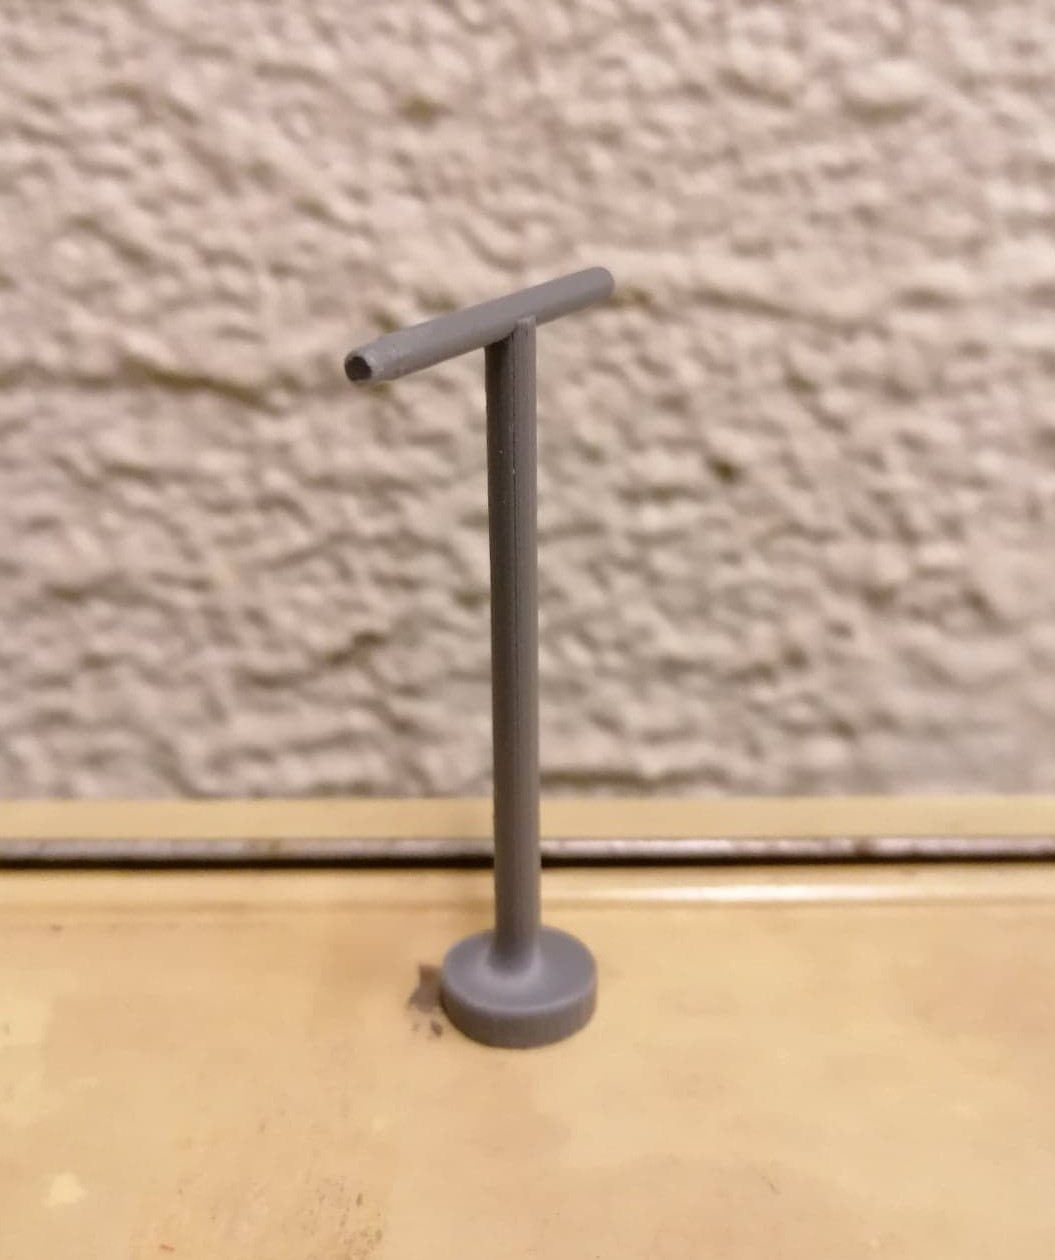
\includegraphics[width=0.5\textwidth]{0_Images/tower.jpg}    
    \caption{The 3D printed tower.}
    \label{fig:towers}
\end{figure}


\subsection{Actuator disk design}
The \gls{AD}s were designed with a diameter of 45 mm, to match the \gls{RWTM}s. The disks were 2.5 \si{\mm} thick.

Two different designs of \gls{AD}s were tested. The first has numerous equally-sized holes spread symmetrically around the center point of the disk, as seen in figure \ref{Fig:holes60} and \ref{Fig:holes40}. It is quite similar to the design of Blackmore et al (2013) \cite{Blackmore2013}. The design is also meant to be similar to those \gls{AD} designs that consist of a thin metal grid, comparable to a grid turbulence generator, as used by Aubrun et al (2013) \cite{Aubrun2013} and Lignarolo et al (2016)\cite{Lignarolo2016}. This design will be called \gls{holes} going forth. The second design is also symmetric around the center point, but this one has rectangular holes that vary in size with radial distance, increasing in size as the radial coordinate increases, as seen in figure \ref{Fig:spider60} and \ref{Fig:spider40}. Thus, the solidity decreases with radial coordinate, matching the characteristics of an actual WT. This design was used by Camp and Cal (2016 and 2019) \cite{Camp2016} \cite{Camp2019} and by Neunaber \cite{Neunaber}. This design will be called \gls{spider}. 
%(however filled in to avoid sharp corners)


\begin{figure} [h!]
    \centering
    \begin{subfigure}[b]{0.45\linewidth}
        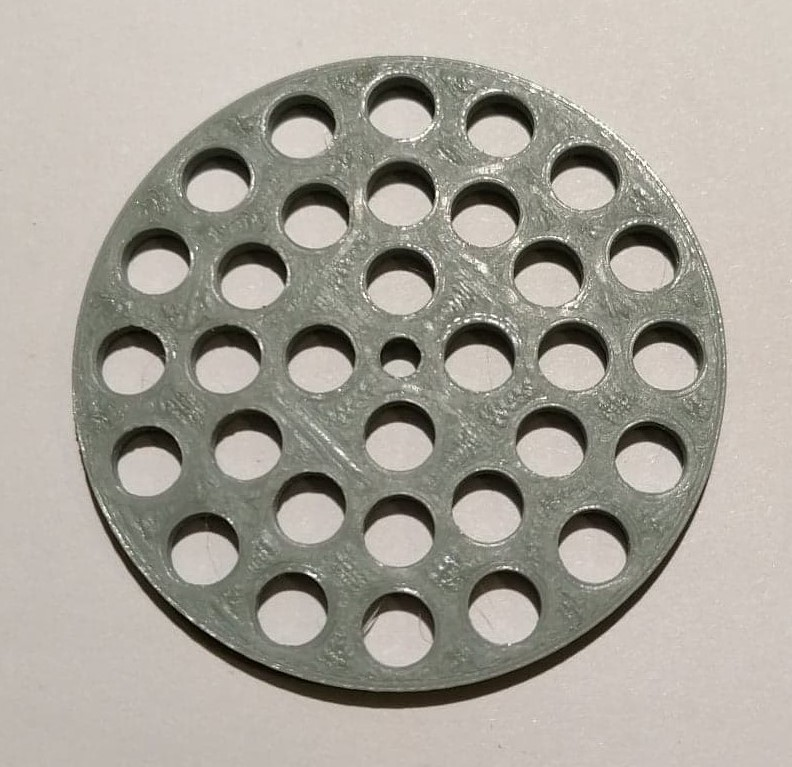
\includegraphics[width=\textwidth]{0_Images/holes60.jpg}
        \caption{The \gls{holes} design}
        \label{Fig:holes60}
    \end{subfigure}
    ~
    \begin{subfigure}[b]{0.45\linewidth}
        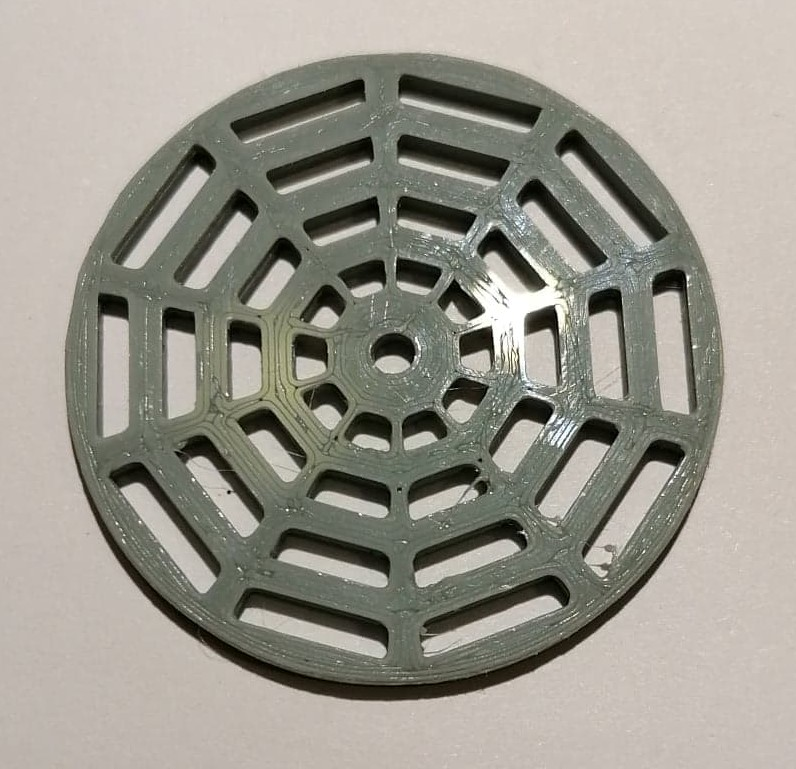
\includegraphics[width=\textwidth]{0_Images/spider60.jpg}
        \caption{The \gls{spider} design}
        \label{Fig:spider60}
    \end{subfigure}
    \caption{\gls{AD}s with a solidity of 60\%.}
    \label{Fig:60Sol}
\end{figure}

\begin{figure} [h!]
    \centering
    \begin{subfigure}[b]{0.45\linewidth}
        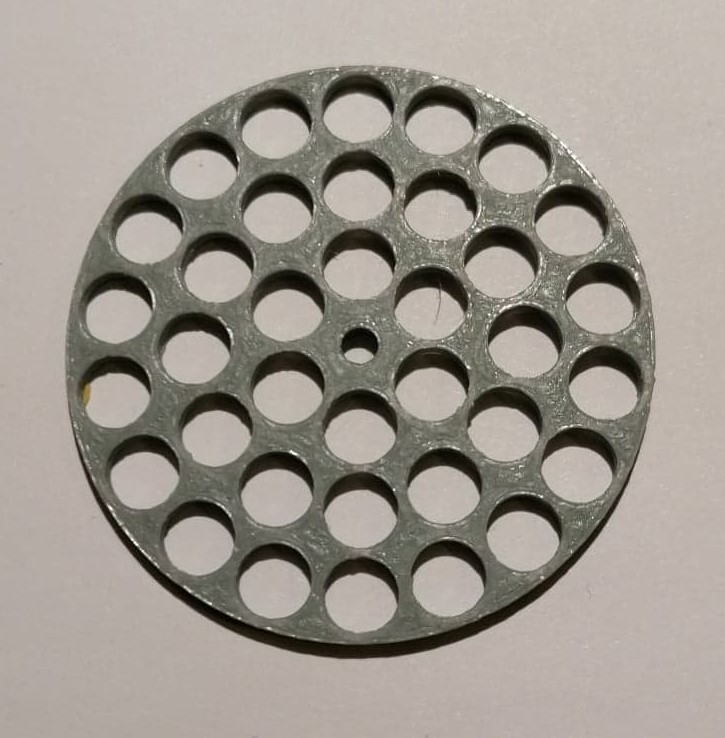
\includegraphics[width=\textwidth]{0_Images/holes40.jpg}
        \caption{The \gls{holes} design}
        \label{Fig:holes40}
    \end{subfigure}
    ~
    \begin{subfigure}[b]{0.45\linewidth}
        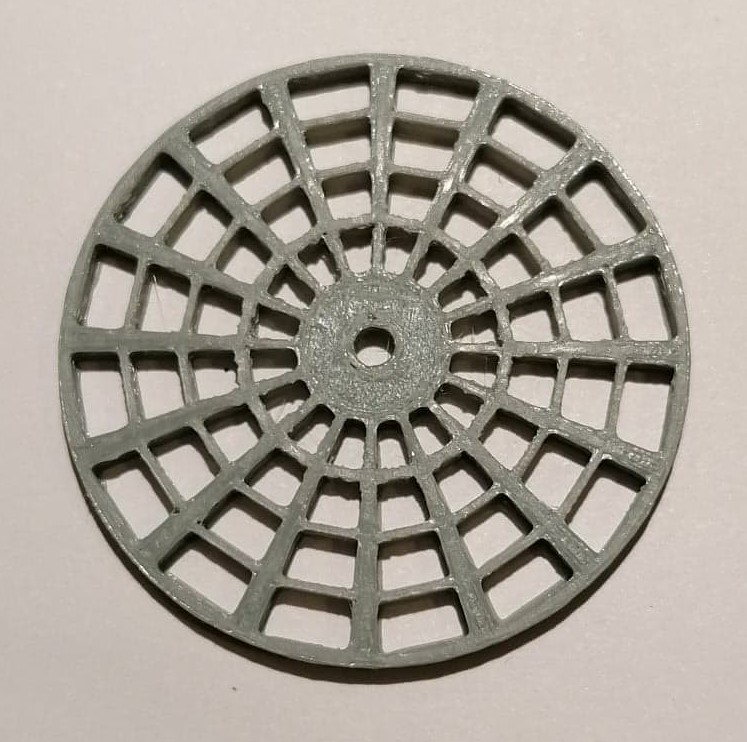
\includegraphics[width=\textwidth]{0_Images/spider40.jpg}
        \caption{The \gls{spider} design}
        \label{Fig:spider40}
    \end{subfigure}
    \caption{\gls{AD}s with a solidity of 40\%.}
    \label{Fig:40Sol}
\end{figure}

For each of these configurations, two solidities were created as an initial try. The chosen values were 60\% and 40\%. A solid disk was also made and tested as a reference case. Three disks of each design and solidity were printed. 

Based on the resulting drag profiles from the initial round of testing, two sets of \gls{AD}s with a solidity of 35\% were designed and made, which can be seen in figure \ref{Fig:holes35} and \ref{Fig:spider35}. The first was made based on the \gls{holes} design. Due to the mentioned limitations regarding the printing thickness, providing a solidity less than 39\% with this design proved problematic. Hence the design was slightly changed, allowing for the holes to also cover the edges of the \gls{AD}s. It was kept in mind that this results in a different disk circumference, and that this might result in a drag force that is not directly comparable to the drag of the previously tested disks with \gls{holes} design. The second disk was made using the \gls{spider} design. 

\begin{figure} [h!]
    \centering
    \begin{subfigure}[b]{0.45\linewidth}
        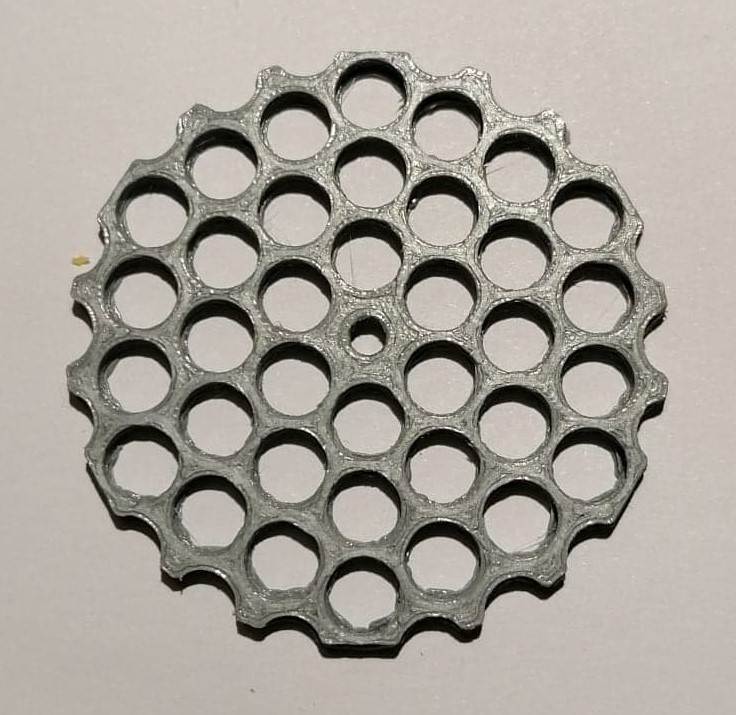
\includegraphics[width=\textwidth]{0_Images/holes35.jpg}
        \caption{The \gls{holes} design}
        \label{Fig:holes35}
    \end{subfigure}
    ~
    \begin{subfigure}[b]{0.45\linewidth}
        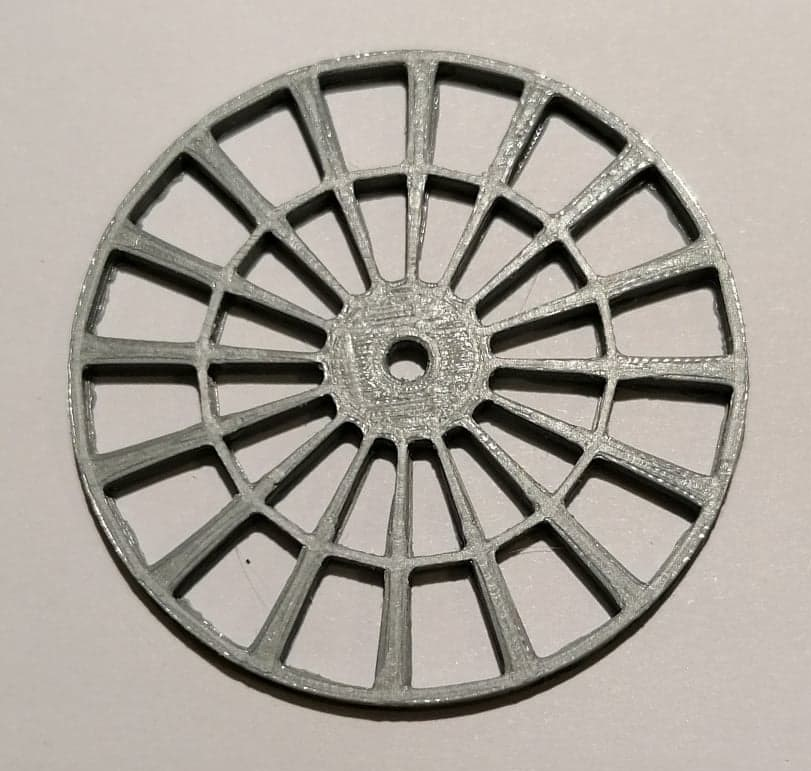
\includegraphics[width=\textwidth]{0_Images/spider35.jpg}
        \caption{The \gls{spider} design}
        \label{Fig:spider35}
    \end{subfigure}
    \caption{\gls{AD}s with a solidity of 35\%.}
    \label{Fig:35Sol}
\end{figure}

Each disk was as mentioned made with a small hole in the center, used to connect the disks to the tower. Thus, this hole was filled in during the tests in the wind tunnel, and did not affect the solidity. This connection resulted in a larger solidity in the center of the disks, which can be argued to represent the nacelle of a wind turbine. A disk connected to a tower can be seen in figure \ref{Fig:towerAndAD}. 



\begin{figure}
    \centering
    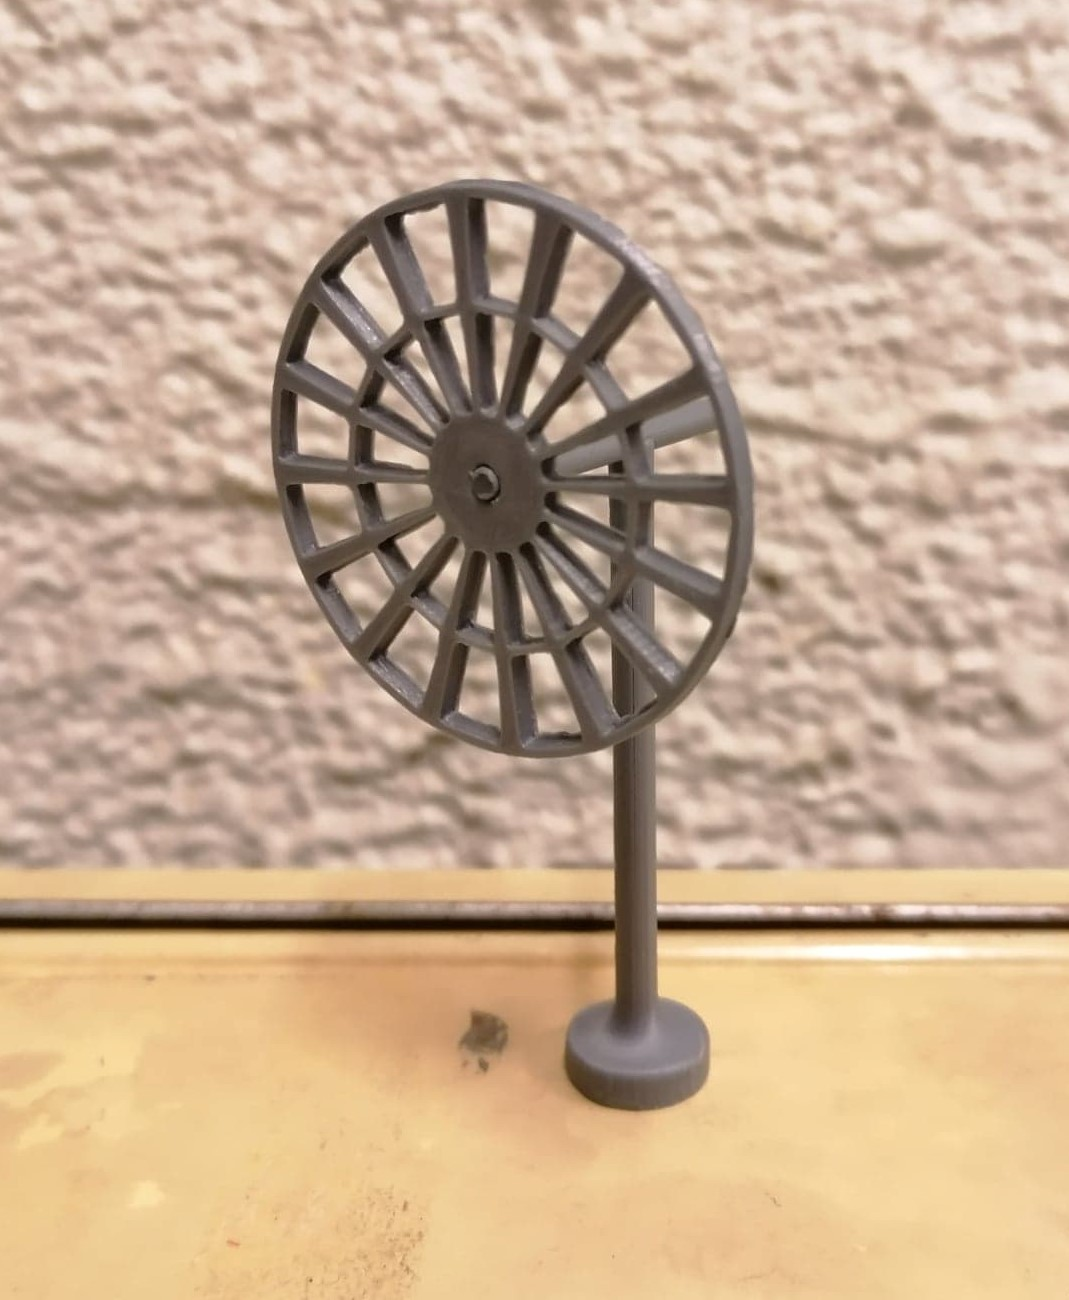
\includegraphics[width=0.5\textwidth]{0_Images/baseAndAD.jpg}    
    \caption{The 3D printed tower connected to the 3D printed \gls{spider} disk with 35\% solidity.}
    \label{Fig:towerAndAD}
\end{figure}

\FloatBarrier

%was made as the designs with rectangular holes that vary in size with radial distance.  

%PICTURE OF DISKS AND TOWER 
%there was a limit to how low the solidity could get, and 
%unrelated